% -*- latex -*-
%-----------------------------------------------------------------------
%;  Copyright (C) 2002
%;  Associated Universities, Inc. Washington DC, USA.
%;
%;  This program is free software; you can redistribute it and/or
%;  modify it under the terms of the GNU General Public License as
%;  published by the Free Software Foundation; either version 2 of
%;  the License, or (at your option) any later version.
%;
%;  This program is distributed in the hope that it will be useful,
%;  but WITHOUT ANY WARRANTY; without even the implied warranty of
%;  MERCHANTABILITY or FITNESS FOR A PARTICULAR PURPOSE.  See the
%;  GNU General Public License for more details.
%;
%;  You should have received a copy of the GNU General Public
%;  License along with this program; if not, write to the Free
%;  Software Foundation, Inc., 675 Massachusetts Ave, Cambridge,
%;  MA 02139, USA.
%;
%;  Correspondence concerning AIPS should be addressed as follows:
%;          Internet email: aipsmail@nrao.edu.
%;          Postal address: AIPS Project Office
%;                          National Radio Astronomy Observatory
%;                          520 Edgemont Road
%;                          Charlottesville, VA 22903-2475 USA
%-----------------------------------------------------------------------
%Body of intermediate AIPSletter for 31 December 2001

\documentclass[twoside]{article}
\usepackage{graphics}

\newcommand{\AIPRELEASE}{June 30, 2002}
\newcommand{\AIPVOLUME}{Volume XXII}
\newcommand{\AIPNUMBER}{Number 1}
\newcommand{\RELEASENAME}{{\tt 31DEC02}}
\newcommand{\OLDNAME}{{\tt 31DEC01}}

%macros and title page format for the \AIPS\ letter.
\input LET98.MAC
%\input psfig

\newcommand{\MYSpace}{-11pt}

\normalstyle

\section{General developments in \AIPS}

\subsection{Linux news: bad compilers}

RedHat has released versions 7.0, 7.1, and 7.2 of their Linux system.
The good news is that version 7.1 and beyond contain numerous system
improvements including the 2.4.2 kernel.  This kernel allows \AIPS\ to
read and write files larger than 2 Gbytes.  The bad news is that these
releases include and depend on the ``GNU compilers version 2.96.''
The quote marks are added because the GNU compiler group never
released a version 2.96 and they do not support this ``version.''  We
have found that this {\tt g77} produces optimized code that is
unreliable.  There are problems with {\tt IMAGR}, TV window setting,
{\tt TVFLG}, and who knows what else.  {\it Furthermore, we have found
that there are problems with GNU's version 3.0.1 through 3.0.4
compilers --- the resultant code is slower and some of it fails.}
We do recommend RedHat release 7.2, but you must also install the GNU
compiler suite version 2.95 (now 2.95.3) ({\it but not GNU gcc
versions 3.0 or later}) and change your local copies of {\tt
FDEFAULT.SH}, {\tt CCOPTS.SH}, and {\tt FDOPTS.SH} to point at it.
Some other Linux distributions also include the 2.96 compiler with the
same unfortunate results. Instructions for fetching and installing the
GNU 2.95.3 compiler are given on the \AIPS\ web page.

\subsection{Current and future releases}

We have reinstated the old practice of having formal \AIPS\ releases,
but on an annual basis with binary releases only for Solaris and
Linux.  All architectures can do a full installation from the source
files.  The next release will be called {\tt 31DEC02} and remains under
development by the (reduced) \AIPS\ Group.  You may fetch and install
a complete copy of this version at any time.  This \Aipsletter\ is
intended to advise you of developments to date in this new release.
Having fetched {\tt 31DEC02}, you may update your installation
whenever you want by running the so-called ``Midnight Job'' (MNJ)
which uses transaction files to copy and compile the code selectively
based on the code changes and compilations we have done.  We expect
users to take the source-only version of {\tt 31DEC02} \AIPS\ over the
Internet (via \emph{anonymous} ftp).

The MNJ has been changed.  The secure shell, with all its fragile
complexities, is no longer required.  Instead {\tt mnj.aoc.nrao.edu}
will serve up \AIPS\ incrementally --- or as a whole --- using the
Unix tool {\tt cvs} running with anonymous ftp.  Linux sites will
almost certainly have {\tt cvs} installed; other sites may have
installed it along with other GNU tools.  Secondary MNJs will still be
possible using {\tt ssh} or {\tt rcp} or NFS as with previous
releases.  We have found that {\tt cvs} works very well, although it
has one quirk.  If a site modifies a file locally but in an
\AIPS-standard directory, {\tt cvs} will detect the modification and
attempt to reconcile the local version with the NRAO-supplied version.
This usually produces a file that will not compile or run as
intended.
\eject

\AIPS\ is now copyright \copyright\ 1995 through 2002 by Associated
Universities, Inc., NRAO's parent corporation, but may be made freely
available under the terms of the Free Software Foundation's General
Public License (GPL)\@.  This means that User Agreements are no longer
required, that \AIPS\ may be obtained via anonymous ftp without
contacting NRAO, and that the software may be redistributed (and/or
modified), under certain conditions.  The full text of the GPL can be
found in the \texttt{15JUL95} \Aipsletter.

\section{Improvements of interest to users in \RELEASENAME}

We expect to continue publishing the  \Aipsletter\ approximately every
six months along with the annual releases.  Despite the reduction in
personnel, there have been a number of changes in {\tt 31DEC02} over
its first six months.  There are three new tasks: {\tt WETHR} to plot
the contents of the weather table including flagging data based on the
contents of the table, {\tt BOXES} to add Clean boxes to a {\tt
BOXFILE} based on source catalogs, and {\tt UVDEC} to copy a \uv\ data
set retaining only every $n^{\uth}$ spectral channel.  There are also
three new verbs: {\tt TKERASE} to clear the contents of the Tektronix
emulation display window, {\tt SG2RUN} to convert the contents of a
{\tt SAVE}/{\tt GET} file into a {\tt RUN} file for use on another
computer and/or user number, and {\tt OUTPUTS} to show those adverbs
whose values will be changed when running the task.  A new {\tt RUN}
file called {\tt WRTPROCS} provides three procedures for automated
writing and reading of FITS disk files.

Other than relatively minor differences, {\tt 31DEC02} is compatible
in all major ways with the 2001, 2000, 1999, and {\tt 15OCT98}
releases.  There are significant incompatibilities with older
versions.

\subsection{Imaging}

\subsubsection{IMAGR}

{\tt IMAGR} and all other tasks that use Clean-component models were
changed to allow up to 4096 fields (or facets).  This change was made
mostly to support multi-resolution Clean, but the previous limit of 512
fields was onerous to some low-frequency observations.

Otherwise, almost all changes to {\tt IMAGR} were in the nature of bug
fixes or very minor improvements.  It defends itself better against
selection of a field with inadequate flux and against bad window
parameters.  The histogram is now done with better resolution and the
{\tt BOXFILE} is copied at the beginning to any new {\tt OBOXFILE}\@.
The multi-resolution Clean algorithm received special attention.  A
bug causing the most important steering parameter to be ignored was
corrected.  The computations of Gaussians were changed to achieve much
improved performance.  {\tt MAXPIXEL} is now allowed to change on a
{\tt TELL} operation.  The first TV display now sets the TV size
correctly and selects the first image to display with improved
information.  The histogram is now computed only over all fields of
the current resolution, {\tt MAXPIXEL} is adjusted with {\tt
IMAGRPRM(16)} for different resolutions, and the actual parameters
used for each resolution are reported.

\subsubsection{BOXES and MFPRT}

{\tt BOXES} is a new task used to convert a source catalog into Clean
boxes to be used with {\tt IMAGR}\@.  It reads any source catalog in
the format used by \AIPS\ for the NVSS and WENSS surveys, allowing one
to start the Clean with boxes around known sources.  {\tt MFPRT} was
changed to offer the option of making an output text file in this
format.  Doing this, one may convert the sources found in a
preliminary imaging followed by {\tt SAD} to a set of boxes to guide a
later round of imaging.

\subsubsection{Other imaging changes}

\begin{description}
\myitem{SAD} and {\tt IMFIT} and {\tt JMFIT} were all corrected and a
             patch issued.  They used the phase center rather than
             the pointing position for the primary beam correction
             and used a linear shift rather than a proper non-linear
             angle for the delay-beam correction.  This had serious
             effects on images well separated from the phase center.
\myitem{REGRD} was overhauled to function correctly on data cubes and
             to provide more sensible defaults for the output
             coordinates.  Some tricks to speed the computations were
             also added.
\myitem{FLATN} was changed to do an unlimited number of pointings,
             although the value to use for {\tt NOISE} for pointings
             in excess of 64 must be taken to be the average of the
             lower numbered ones.
\myitem{MAPBM} was overhauled to image all four Stokes into separate
             planes of a cube and to image each selected antenna into
             a separate output file.
\end{description}

\subsection{VLBI matters}

\subsubsection{New VLBA/VLBI calibration procedures in \AIPS}

With the addition of three procedures, {\tt VLBAUTIL}, a package of
procedures for the reduction of VLBA (and most VLBI) experiments, will
handle most VLBA experiments (including spectral line) from loading
through fringe fitting.  The additional procedures are:
(1) {\tt VLBASRT}, which sorts and indexes a dataset, if needed; (2)
{\tt VLBAFIX}, which will sort, index, split into separate frequency
files, deal with subarrays, and fix polarization labeling, as needed;
and (3) {\tt VLBAMPCL}, which does manual phase-cal corrections on one
or two scans.  {\tt VLBAFIX} is designed to replace 4 procedures which
are already part of the package ({\tt VLBASRT}, {\tt VLBASUBS}, {\tt
VLBAFPOL} and {\tt VLBAFQS}) and can/should be run after loading any
dataset, as it only performs the necessary corrections.  The procedure
which loads VLBA data ({\tt VLBALOAD}) has also been significantly
changed so that it merges {\tt TY}, {\tt GC} and {\tt PC} tables after
the data are loaded.  Formerly it was necessary to run {\tt VLBAMCAL}
after {\tt VLBALOAD} to merge these tables, now it is done
automatically.

For a detailed description on how to use all these procedures see
a recent version of the \AIPS\ \Cookbook, Chapter 9 and Appendix C.

\subsubsection{Other changes}

\begin{description}
\myitem{FITLD} would occasionally report mysterious problems with {\tt
               BA} bandpass tables which are not actually supported on
               the VLBA Correlator data tapes.  This was due to a name
               collision with \AIPS' batch files, so VLBA bandpass
               tables will now be named {\tt BT} should they ever
               appear.  The scaling of the visibilities turns out to
               be different for each of the VLBA, Penticton, and EVN
               correlators, requiring some changes to be made to {\tt
               FITLD}\@.  The VLBA Correlator jobs can have errors
               that cause unexpected {\tt FQ}ids to occur in some
               tables --- those not actually processed in the
               correlator.  Some code to avoid self-destruction was
               added to {\tt FITLD}, although this does not restore
               the calibration data to correctness.
\myitem{CVEL} and {\tt BPASS} were changed to shift the second antenna
               for data from the EVN correlator, while the first
               antenna is used for all others.  Actually, neither
               is shifted at this stage for the VLBA Correlator.
\myitem{FRPLT} was overhauled to allow a wide range of plot options
               for fringe-rate spectra including multiple plots per
               page, multiple time intervals per baseline, multiple
               IFs and/or polarizations together as one long spectrum,
               and many more.
\end{description}

\subsection{UV data handling and calibration}

\subsubsection{WETHR, INDXR, and FILLM}

In the previous release, {\tt FILLM} was given the ability to compute
initial values for {\tt CL} table 1 to correct for the antenna gains
and atmospheric opacity.  In the present release, these computations
were improved with minor improvements to the opacity and vapor
pressure computations.  A new ``seasonal'' average opacity model was
added, along with an option to use a weighted average of the seasonal
opacity and the opacity computed from the surface weather
measurements.  The two methods are averaged equally by default.  The
{\tt HELP} file was improved and the history file now records some of
what was done.  An addressing bug was corrected for the gains averaged
over antenna.

{\tt INDXR} was revised to be able to redo the opacity and gain
corrections done by {\tt FILLM} while writing a new {\tt CL} table 1.
This requires the weather table to have been written with a short time
interval but otherwise removes the dependence on tapes and {\tt
FILLM} in case the {\tt CL} table 1 is lost or did not contain the
corrections.

{\tt WETHR} is a new task that will plot a wide range of parameters
read or computed from the weather ({\tt WX}) table now provided with
both VLA and VLBA data.  The same parameters that can be plotted may
be used to flag the visibility data.  {\tt WETHR} uses the same
subroutines as {\tt FILLM} and {\tt INDXR} to compute relative
humidity, water column in mm, and zenith opacities at K and Q bands.

\subsubsection{Other changes}

\begin{description}
\myitem{SPLAT} was corrected for a bug that arose when channel
               averaging was being done.  If the number of channels
               specified by the {\tt BCHAN} to {\tt ECHAN} range was
               not an exact multiple of {\tt CHANNEL}, then a data
               addressing error affecting the IFs after the first was
               possible.  The output data for those IFs were simply
               wrong.  A patch for this was announced.
\myitem{POSSM} was corrected to plot and label properly multi-IF plots
               and the option to include multiple polarizations in one
               long, correctly labeled, spectrum was added.  It can
               also loop over polarizations.  Bandpass plotting was
               corrected.
\myitem{DEFLG} was corrected to handle 4-polarization input files and
               to do time integration correctly.  It used all of the
               times which was fine in a test dataset but not in the
               real world.
\myitem{BPASS} was given the option to normalize after the scan
               average of the data which is less biased than
               normalizing on a record-by-record basis.  {\tt SOLINT}
               defaults to infinity for single-source files rather
               than dividing by zero.
\myitem{DBCON} was changed to concatenate {\tt TY} and {\tt WX} tables
               as it already does {\tt CL} and {\tt FG} tables.
\myitem{CLIPM} was corrected to use the {\tt ANTENNAS} and {\tt
               BASELINE} adverbs which a typo caused it to ignore.
\myitem{UVDEC} is a new task to copy every $n^{\uth}$ spectral channel
               of a \uv\ dataset.  Frequency-smoothing operations done
               by other tasks do not decrement the number of channels
               while other tasks average channels while decrementing.
\myitem{UVMOD} was corrected to compute RL and LR models properly.
\end{description}

\subsection{Miscellaneous matters}

\begin{description}
\myitem{WRTPROCS} \hspace{1em} is a new {\tt RUN} file which contains 3
           procedures. {\tt FITDISK} writes FITS disk files with names
           reflecting the \AIPS\ logical names.  {\tt WRTDISK} writes
           FITS disk files with standardized names which can then be
           read back by {\tt READISK} looping through numerous files.
           These procedures are meant to assist in backing up data and
           in transferring data between computers, particularly
           computers of dissimilar architecture (\eg\ PCs and SUNs).
\myitem{TKERASE}\hspace{0.2em} is a new verb to erase the
           Tektronix-emulation display.  If a plot is left in the
           display, then any expose event on the window causes the
           full plot to be redrawn. This can occupy the computer for
           some time during which the user can only wait.
\myitem{SG2RUN} is a new verb to convert the current copy of the {\tt
           AIPS} vocabulary to a text file suitable to be {\tt RUN} on
           another computer and/or for another user number.  A {\tt
           GET\ {\it SGname} ; OUTFILE = {\it out\_name} ; SG2RUN}
           will convert a particular {\tt SAVE}/{\tt GET} file into a
           text file, enabling the full contents, including procedure
           definitions and adverb values, to be transferred elsewhere.
\myitem{TACOP} was changed to copy any type of extension file.
           Previously, it would try to copy {\tt PL} and other
           non-table extension files, but it would fail to do it
           properly.
\myitem{External} file naming has been changed to allow adverbs such
           as {\tt INFILE} to contain the actual file name with
           directories rather than requiring a logical (or
           environment) variable name.  FITS disk files will again
           default to the {\tt \$FITS} area unless a logical name or a
           full path name (starting with a {\tt /}) are given.
\myitem{\Cookbook} chapters have been updated to mention changes in
           the VLBI procedures, {\tt PRTAB}, {\tt BOXES}, {\tt SAD}
           {\it et al.}, {\tt RMSD}, {\tt WETHR}, and more.  Appendix
           C was overhauled to emphasize the VLBA procedures rather
           than the older ways of doing things.  A new appendix D on
           high frequency observing and data reduction techniques was
           added.  The previous Appendix D is now called Appendix F\@.
\myitem{PRTAB} was given the adverb {\tt NDIG} to tell it whether
           normal or extended precision is needed in its displays of
           floating-point columns.
\myitem{All sky} plotting of coordinates had some problems which were
           corrected.
\myitem{UVCON} was given the option to multiply the input model by the
           single-dish primary beam pattern including a shift useful
           for simulating mosaic observations.  It can read antenna
           positions in up to 4 different coordinate systems.
\end{description}

\subsection{Adverb pass-back and other programmer tidbits}

Adverb values may now be passed back to {\tt AIPS} by tasks.  Each
adverb listed in the {\tt INPUTS} section of a {\tt HELP} file has a
code character in column 10 which tels {\tt AIPS} what to do with it.
An adverb is used by {\tt GO} (and {\tt INPUTS}) and/or {\tt TELL}
(and {\tt SHOW}) and/or the value pass-back (and the new verb {\tt
OUTPUTS})\@.   The codes are
\begin{center}
\begin{tabular}{llll}
{\tt '\ '} & {\tt GO} &            & \\
{\tt '*'}  & {\tt GO} & {\tt TELL} & \\
{\tt '?'}  & {\tt \ } & {\tt TELL} & \\
{\tt '\&'} & {\tt GO} & {\tt TELL} & pass-back \\
{\tt '\%'} & {\tt \ } & {\tt TELL} & pass-back \\
{\tt '\$'} & {\tt GO} &            & pass-back \\
{\tt '@'}  & {\tt \ } &            & pass-back \\
\end{tabular}
\end{center}
If {\tt GO} detects an adverb calling for pass-back, it runs the task
in {\tt DOWAIT 1} mode and then reads back the changed adverb values
from the task communication ({\tt TD}) file.  The subroutine {\tt
PTPARM} is used by the task to put the adverb values back in the file
as a consecutive array of $n$ values.  Since the adverbs involved may
not be consecutive in the inputs to the task (or even in the inputs),
some care is obviously required.

Note that the verbs {\tt INP} and {\tt INPUTS} only display the
adverbs associated with {\tt GO}; the verb {\tt SHOW} only displays
the adverbs associated with {\tt TELL}; and the new verb {\tt OUTPUTS}
only displays the adverbs associated with adverb value pass-back.  At
present, the only task that implements this capability is {\tt IMEAN},
which passes back the fitted rms and mean.

{\tt XAS.SHR} was changed in a subtle way to allow the standard Unix
utility {\tt sh} to unpack the file into its component parts.  The
{\tt UNSHR} program is no longer needed although it is still used for
now.

\section{Recent \AIPS\ and related Memoranda}

The following new \AIPS\ Memoranda are available from the \AIPS\ home
page.

\newcommand{\KR}{{$\tt KRING$}}
\newcommand{\FR}{{$\tt FRING$}}
\begin{tabular}{lp{5.8in}}
107 &   {\tt KRING} versus {\tt FRING} Tests \\
   &    Amy J. Mioduszewski (NRAO)\\
   &    April 8, 2002\\
   &    This comparison was designed to discover whether \KR\ or \FR\
should be used for most, if not all, fringe fitting problems.  Within
reasonable uncertainty, \FR\ and \KR\ performed very similarly.  There
is some indication that the default signal to noise cutoff in \KR\ is
too low for low signal to noise cases.  As one would expect, for high
flux density sources the solution interval should be set as low as
possible.  For low flux density sources the solution interval should
be set considering both the ability to find a good solution and to
interpolate accurately.  The only consistent difference between \KR\
and \FR\ is that \KR\ runs faster than \FR\ a vast majority of the
time, typically by factors of 1.5 to 4.
\end{tabular}

\section{VLBA data calibration pipeline}

\begin{figure}
\centerline{\resizebox{!}{4.5in}{\includegraphics{Let02A.LSb}%
    \hspace{3em}\includegraphics{Let02A.LSc}}}
\caption{The algorithm chain and the options list.}
\end{figure}

Currently we are working on a VLBA data calibration pipeline, as a
{\tt RUN}-file in \AIPS\ that is primarily based on the {\tt
VLBAUTIL} procedures. It is intended to perform the calibration tasks
and make lots of plots and some simple images to find out whether the
calibration has worked --- it is not supposed to perform the art of
high-fidelity imaging for you. Eventually, the VLBA data calibration
pipeline will be available to \AIPS\ users as part of the \AIPS\
distribution and the MNJ\@.  We will soon advertise its peculiars and
how to obtain a copy and its use on a web page under the VLBA's
calibration section.

At the moment the VLBA data calibration pipeline works reasonably well
for simple VLBA-only experiments correlated in Socorro, at frequencies
between about 1 and 15 GHz, both for (pseudo-)continuum and spectral
line experiments. It has been run successfully on higher and lower
frequencies, but we're not advertising that yet --- in particular
the spectral RFI flagging must be improved. The VLBA data calibration
pipeline is expected to be extended to work at a wider range of
frequencies, to do polarization calibration and more robust data
flagging, and to include non-VLBA antennas (in particular the
single-dish VLA, GBT, and EB). Keep watching the VLBA data calibration
web page for progress reports.

We're starting to run the VLBA data calibration pipeline on every
suitable experiment and investigating its use and performance and how
to distribute the calibrated multi- and single-source UVFITS files to
the users. Images and calibration plots will not be distributed, they
are only produced to check the calibration before we distribute the
data to the PI\@. As we distribute single-source UVFITS files, the
user could import the files into his/her favorite imaging package
(\eg\ aips++, difmap) without the need to use \AIPS\@.

The VLBA data calibration pipeline will be invoked (after it has been
added to \AIPS) by issuing the procedure {\tt RUN} command defining
the procedures. The user interface is, as for any other task in \AIPS,
an input table with the options available (and an explanatory {\tt
HELP}-file). At the start of the VLBA data calibration pipeline, the
procedure checks the inputs, for which there are no defaults, and
bombs immediately if there are errors or unexpected values. If
everything is okay, the procedure starts reading the Socorro
correlator distribution tape (or from a pre-loaded file), and performs
the calibration, fringe-fitting, and imaging as shown in Figure 1,
making plots of the most essential steps on the fly, which can be
investigated easily after the procedure has finished. Note that there
is some coarse flagging done, as well as a bandpass calibration (also
for continuum) and an ionospheric electron content correction. The
procedure, once it starts, loops over the different frequency bands,
and ends when all the images are made. There are several options, such
as survey calibration (large number of sources to be fringe fitted),
phase-referencing schemes, and an optional self-cal (which is not yet
very robust). More options and improvements are likely to be
implemented later.

If, at the end, it turns out that something went wrong, it is very
easy to redo the VLBA data calibration pipeline, \eg\ after some extra
flagging, without the need to reload the data. Remember that when the
VLBA data calibration pipeline starts, it does not need any user
interaction until it is done, so no matter how long fringe-fitting
takes, the user can concentrate on other things while the VLBA data
calibration pipeline is running in a background \AIPS\ window.

\section{\AIPS\ Distribution}

The web site for downloading the {\tt 31DEC01} version of \AIPS\ as
well as the {\tt 31DEC02} development version was moved to the NRAO
Array Operations Center in Socorro, NM\@.  Unfortunately, as of this
writing, no logging tools are in place to keep track of how many sites
have downloaded these versions of \AIPS, nor of how many sites are
currently running the ``Midnight Job.''  It is clear that some sites
run the Midnight Job from accounts for which no one reads the
resulting e-mail  There are currently at least two sites which are
running MNJs that do not work.  We receive copies of the error
messages on a daily basis (in one case), but are powerless to contact
the culprits since no one is reading e-mail sent to the account
running the MNJ\@.  Please test your MNJ interactively and read the
consequent e-mails.

The MNJ encountered a few difficulties with {\tt cvs} early on and, at
a somewhat later time, one site helped us uncover a subtle problem in
timing.  The former have been fixed by our {\tt cvs}-guru, while the
latter was corrected by having the NRAO provide the time information
to be associated with any particular run of the MNJ\@.  No matter when
you run the MNJ, the time stamp in the {\tt LASTGOOD.DAT} {\it et
al.}~ files will be the time stamp at which the NRAO {\tt cvs} master
synchronized itself.

\section{Patch Distribution for {\tt 31DEC01}}

As before, important bug fixes and selected improvements in
\OLDNAME\ can be downloaded via the Web beginning at:

\begin{center}
\vskip -10pt
{\tt http://www.cv.nrao.edu/aips/patch.html}
\vskip -10pt
\end{center}

Alternatively one can use {\it anonymous} \ftp\ on the NRAO cpu {\tt
aips.nrao.edu}.  Documentation about patches to a release is placed
in the anonymous-ftp area {\tt pub/aips/}{\it release-name} and the
code is placed in suitable subdirectories below this.   Information on
patches and how to fetch and apply them is also available through the
World-Wide Web pages for \hbox{\AIPS}.  As bugs in \RELEASENAME\ are
found, they are simply corrected since \RELEASENAME\ remains under
development.  Corrections and additions are made with a midnight job
rather than with manual patches.  Remember, no matter when you
received your copy of \OLDNAME\ {\it you must} fetch and install its
patches if you require them.

The \OLDNAME\ release had a few important patches including a new one
in late June.  These were:
\begin{enumerate}
\item\ {\tt SAD}, {\tt JMFIT}, and {\tt IMFIT} fail to handle the
      primary beam correction properly for offset fields {\it
      2002-02-11}.
\item\ {\tt IMAGR} failed to apply the {\tt IMAGRPRM(11)} parameter to
      the peak in the Clean windows {\it 2002-02-19}.
\item\ {\tt SPLAT} failed to average spectral channels properly for
      multiple IFs {\it 2002-06-20}.
\end{enumerate}
\vfill\eject

% Order form and mailer page
%\cleardoublepage
\pagestyle{empty}
%\centerline{\resizebox{!}{23.3cm}{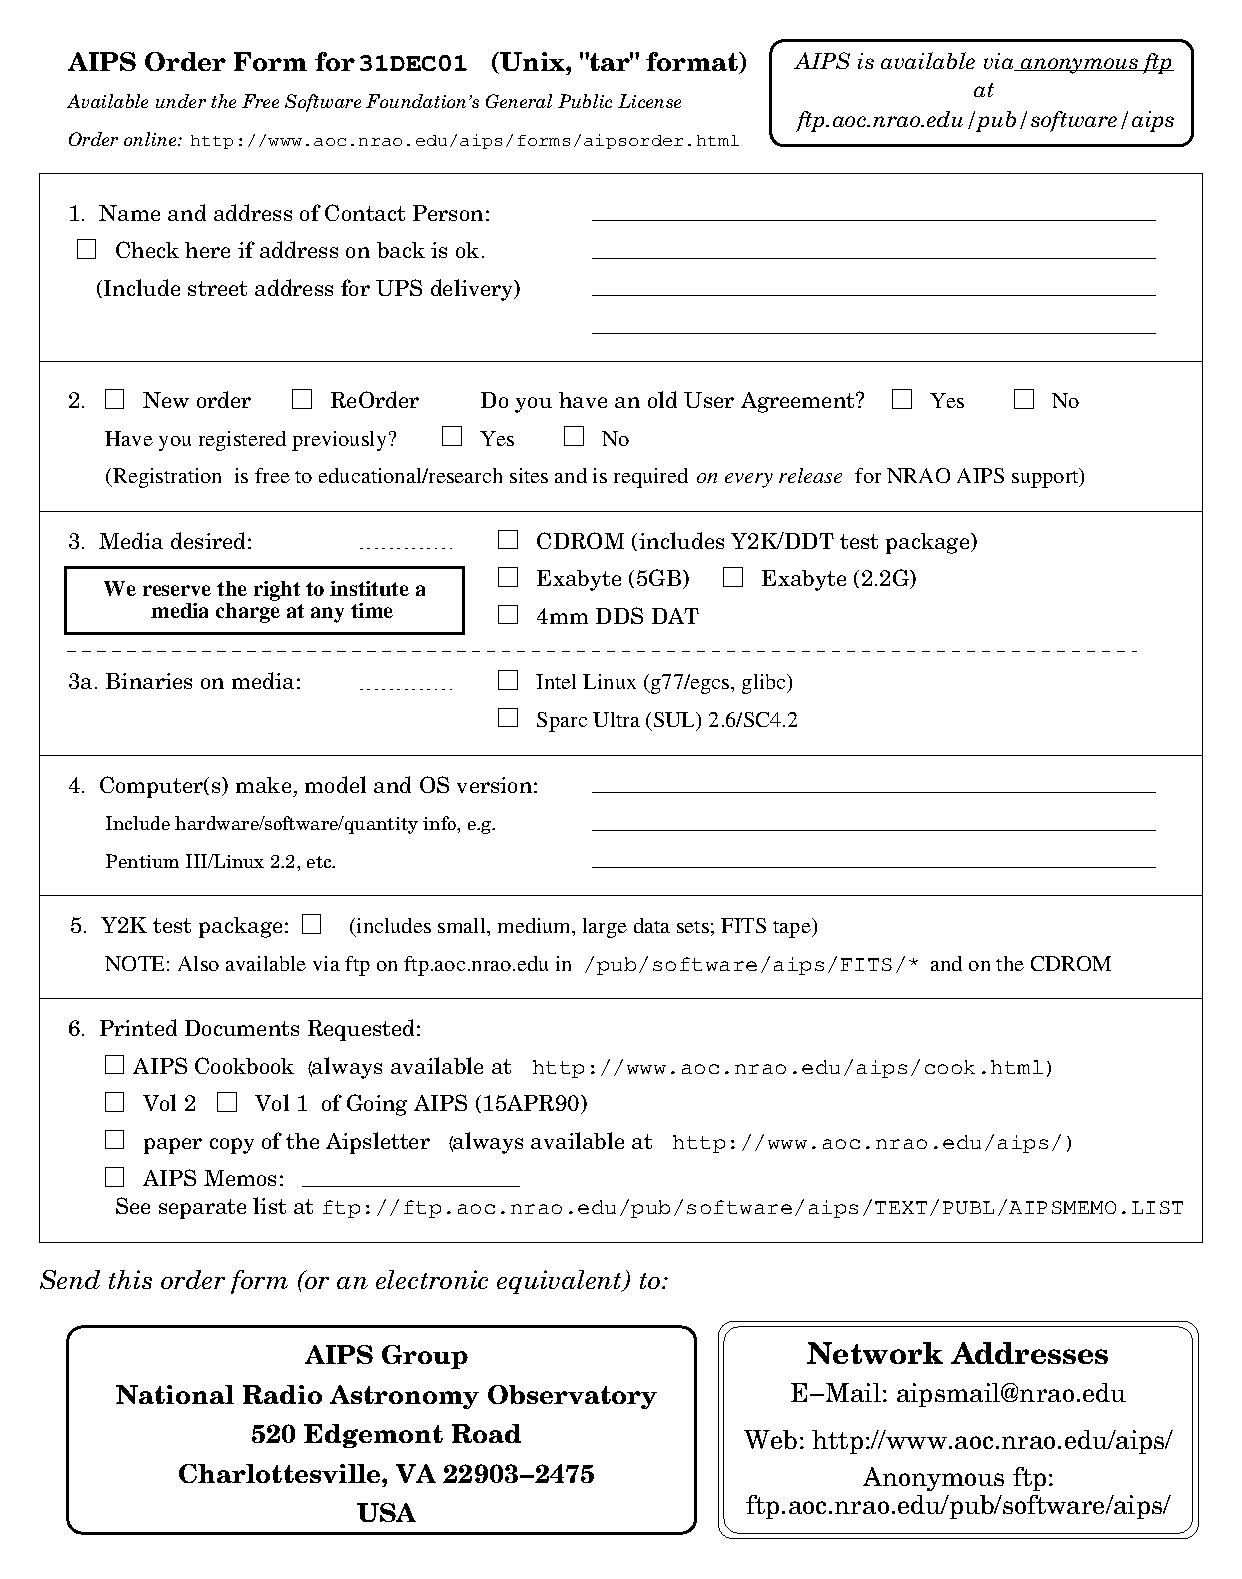
\includegraphics{FIG/AIPSORDER.PS}}}
% \vfill\eject
 \vbox to 4.4in{
  \vfill
  \centerline{\resizebox{!}{2.6in}{\includegraphics{FIG/Mandrill.eps}}}
  \vspace{12pt}
  \centerline{{\huge \tt \AIPRELEASE}}
  \vspace{12pt}
  \vfill}
\phantom{...}
\centerline{\resizebox{!}{!}{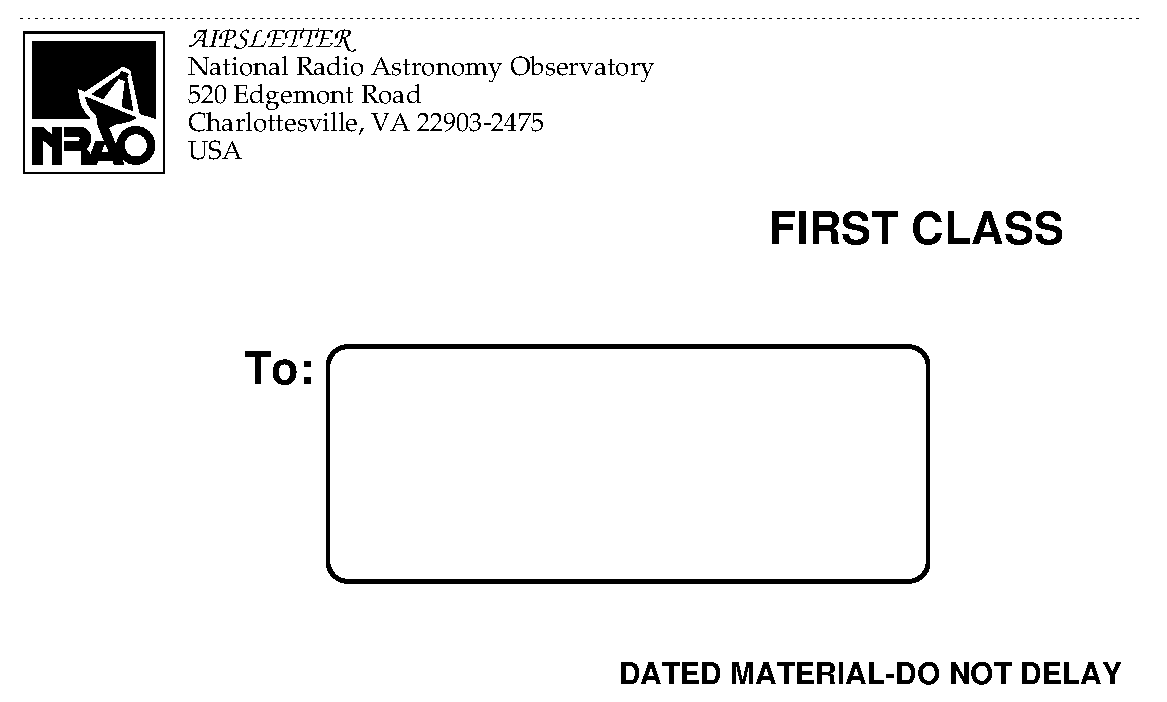
\includegraphics{FIG/AIPSLETM.PS}}}

\end{document}
